\section{Công cụ Joern}

\subsection{Đặc tả đồ thị thuộc tính mã nguồn của Joern}

% Dự án CPG [6, 8] cho phép biểu diễn mã nguồn của các ngôn ngữ lập trình khác nhau dưới dạng đồ thị. Cho đến nay, trọng tâm là Java và C/C++ nhưng có hỗ trợ thử nghiệm cho Python, Go và TypeScript. Mục tiêu của dự án là cung cấp một cách biểu diễn mã nguồn không phụ thuộc vào ngôn ngữ. Hơn nữa, thư viện CPG cung cấp một cách để lưu trữ đồ thị trong neo4j, và truy cập đồ thị thông qua giao diện dòng lệnh. Thư viện CPG được thiết kế để cho phép tái sử dụng các truy vấn chung cho tất cả các ngôn ngữ lập trình được hỗ trợ. Để đạt được mục tiêu này, thư viện CPG định nghĩa một hệ thống phân cấp lớp đầy đủ, bao gồm các loại câu lệnh và biểu thức khác nhau. CPG chứa thông tin như hệ thống kế thừa của mã nguồn, đồ thị luồng điều khiển và đồ thị lời gọi hàm, đồ thị phụ thuộc dữ liệu. Thiết kế hiện tại chủ yếu nhắm vào các ngôn ngữ lập trình hướng đối tượng. Để đối phó với khả năng thiếu một số đoạn mã hoặc lỗi trong mã, thư viện có khả năng chịu lỗi với mã không đầy đủ, không biên dịch được và thậm chí ở mức độ nào đó còn không chính xác.

Với định nghĩa về đồ thị thuộc tính mã nguồn được đề ra, đồ thị thuộc tính mã nguồn đã được nghiên cứu rộng rãi và có rất nhiều phiên bản cài đặt được xây dựng dành cho các mục đích khác nhau \cite{ xiaomeng2018cpgva, kuchler2022representing, weiss2022language, keirsgieter2020graft}. Tuy nhiên có một phiên bản được do chính tác giả của định nghĩa đồ thị thuộc tính mã nguồn, Fabian Yamaguchi, đích thân phát triển và mã nguồn mở mang tên Joern \cite{joernJoernHunteraposs}.

Các thành phần trong đồ thị thuộc tính mã nguồn theo đặc tả CPG của Joern bao gồm nút, cạnh, và thuộc tính. Các nút đại diện cho các thành phần cấu trúc của chương trình bao gồm như phương thức, biến, và cấu trúc điều khiển. Mỗi nút có một loại riêng, loại này chỉ ra loại cấu trúc chương trình mà nút đó đại diện. Ví dụ, một nút với loại METHOD đại diện cho một phương thức, trong khi một nút với loại LOCAL đại diện cho khai báo của một biến cục bộ. Cạnh thể hiện quan hệ giữa các thành phần cấu trúc chương trình, cạnh này là có hướng và có nhãn. Ví dụ, để biểu thị rằng một phương thức chứa một biến cục bộ, chúng ta có thể tạo một cạnh với nhãn CONTAINS từ nút phương thức đến nút biến cục bộ. Bằng cách sử dụng các cạnh có nhãn, có thể biểu diễn nhiều loại quan hệ khác nhau trong cùng một đồ thị. Hơn nữa, các cạnh có hướng để biểu thị mối quan hệ có chiều, ví dụ rằng phương thức chứa biến cục bộ nhưng không xảy ra điều ngược lại. Giũa hai nút có thể tồn tại nhiều cạnh. Các nút, cạnh có các thuộc tính, tồn tại dưới dạng khóa và giá trị, trong đó các khóa phụ thuộc vào loại nút, nhãn cạnh riêng biệt. Đồ thị thuộc tính mã nguồn được lưu trữ trong một cơ sở dữ liệu đồ thị và khai thác thông qua một ngôn ngữ truy vấn đặc thù dựa trên Scala.

Một phiên bản cài đặt cụ thể của đồ thị thuộc tính mã nguồn sẽ định nghĩa các loại nút, loại cạnh, thuộc tính và quan hệ giữa chúng, ngoài ra có thể bao gồm các mở rộng khác. Định nghĩa về cạnh, nút có thể được chuyên biệt cho một ngôn ngữ cụ thể hoặc tổng quát cho nhiều ngôn ngữ. Đồ thị thuộc tính mã nguồn của Joern được thiết kế chủ yếu cho C/C++ và Java, và cũng có hỗ trợ ngôn ngữ lập trình khác như Python, Go, TypeScript, ... Tuy nhiên hiện tại Joern chưa hỗ trợ cho ngôn ngữ Rust.

Đặc tả CPG của Joern được thiết kết chủ yếu cho ngôn ngữ C/C++ và Java, đưa ra định nghĩa CPG cho các cấu trúc chung như if else, switch case, while, for, ... mà nhiều ngôn ngữ khác có cấu trúc ánh xạ tương đồng. Dù vậy, chuẩn chung này không thể đáp ứng được nhu cầu của tất cả các ngôn ngữ. Joern tập trung cho 2 ngôn ngữ lớn là C/C++ và Java do vậy sẽ đặc tả hiện tại sẽ phù hợp với các ngôn ngữ có cú pháp C-like và hướng đối tượng. Trong khi đó Rust là một ngôn ngữ lập trình mới, có cú pháp dựa trên C-Like nhưng vẫn có đôi chút sự khác biệt vì đây là ngôn ngữ hiện đại, hỗ trợ đan xen cả hướng đối tượng và hướng hàm. Đặc biệt với tính hướng hàm, Rust có nhiều cú pháp mới mà Joern chưa hỗ trợ, hay những biểu thức, mệnh đề trong C/C++ hay Java là không hợp lệ nhưng ngược lại đối với Rust. Nhìn chung bản đặc tả CPG của Joern là một cơ sở bao phủ các tính năng phổ biến xuất hiện trong nhiều ngôn ngữ nhưng không thể đáp ứng được tất cả, đặc biệt là các ngôn ngữ lập trình hiện đại. Do vậy đối với từng ngôn ngữ riêng biệt vẫn phải bổ sung thêm các định nghĩa mới cho phù hợp với từng ngôn ngữ. Đặc biệt đối với Rust, cơ chế quản lý bộ nhớ an toàn thể hiện qua các tính năng ownership, borrowing, lifetime là thứ Joern chưa có.

\subsection{Luồng hoạt động của công cụ Joern}
\label{sec:joern_flow}

\begin{figure}[H]
  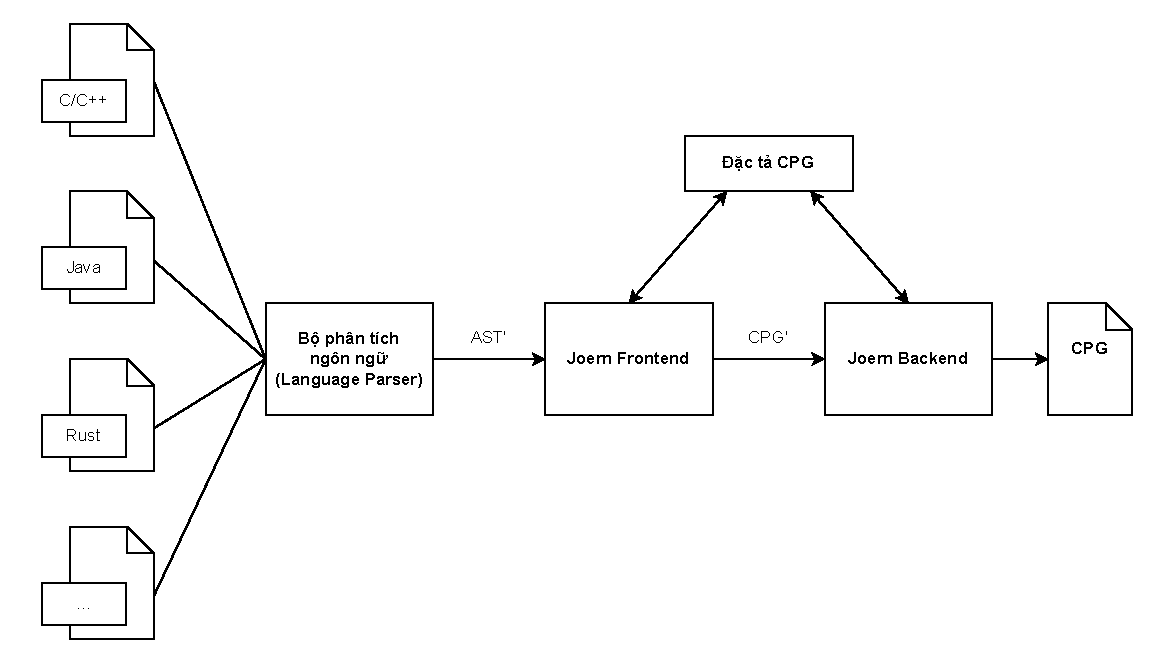
\includegraphics[width=1\columnwidth]{figures/c2/c2_frontend_backend.drawio.pdf}
  \centering
  \caption{Cách hoạt động của công cụ Joern.}
  \label{img:c2_frontend_backend}
\end{figure}

Ngoài phần đặc tả CPG dùng chung cho nhiều ngôn ngữ, Joern còn cung cấp 1 kiến trúc cài đặt thực tế có tính mở rộng cao. Joern hiện tại hỗ trợ rất nhiều ngôn ngữ C/C++, Java, Python, Go, TypeScript, ... Để đáp ứng được nhiều ngôn ngữ và đồng thời mở rộng cho các ngôn ngữ khác trong tương lai, kiến trúc của Joern bao gồm 2 thành phần chính là Joern Frontend và Joern Backend, đây là 2 thành phần có tính tái sử dụng cao, không phụ thuộc vào ngôn ngữ đầu vào. Luồng hoạt động dựa trên kiến trúc Joern sẽ được trình bày như sau.

Mỗi ngôn ngữ có tập các cú pháp khác nhau, tương ứng cũng sẽ có định nghĩa về cây AST khác nhau, đây là phần người dùng muốn mở rộng Joern cho 1 ngôn ngữ mới cần phải tự đảm nhiệm. Bước đầu, mã nguồn của 1 ngôn ngữ được công cụ Language Parser chuyển thành cây AST*. Cây AST* ở đây không nhất thiết chỉ dừng ở đúng mức độ thông tin là 1 cây AST mà có thể bổ sung thêm thông tin khác như kiểu dữ liệu, vị trí nút tương ứng trong mã nguồn, ... nhưng đảm bảo đủ thông tin là 1 cây AST tối thiểu. Ví dụ như các ngôn ngữ có sự phát triển lâu dài như C/C++ sử CDT \cite{eclipseEclipseCC} để làm Language Parser. CDT là công cụ lớn, được dùng trong các IDE nên số lượng thông tin khai thác được rất đáng kể. Còn những ngôn ngữ hiện đại như Rust, thì các công cụ như này chưa được phát triển toàn diện nên thông tin của cây AST* chưa được đầy đủ.
Tiếp theo, cây AST* sẽ được biến đổi thành đồ thị thuộc tính mã nguồn theo định nghĩa trong đặc tả CPG. Đây là công việc của Joern Frontend. Joern Frontend sẽ đọc cây AST* và chuyển đổi thành đồ thị thuộc tính mã nguồn theo đặc tả CPG. Joern Frontend đối với từng ngôn ngữ cũng là phần cần làm riêng, thực tế công việc cần làm là chuyển đổi cấu trúc dữ liệu của cây AST* sang cấu trúc dữ liệu tương ứng của định nghĩa CPG. Joern Frontend đóng vai trò chuyển đổi cây AST* sang đồ thị CPG*.

Sau khi được Joern Frontend xử lý, ta sẽ có được đồ thị CPG* nhưng đồ thị CPG* này là đồ thị không hoàn chỉnh. Để hoàn thiện được đồ thị CPG* thì ta cần phải sử dụng đến Joern Backend. Ở Joern Frontend, ta đã thực hiện bước chuyển đổi 1 nút AST thành 1 nút CPG, tạo thêm các cạnh để thể hiện các mối quan hệ giữa các nút, tuy nhiên các cạnh này chưa thể hiện được đầy đủ đồ thị CPG bao gồm AST, CFG, PDG. Với cấu trúc dữ liệu CPG của Joern, ta chỉ cần định nghĩa 1 phần số cạnh, nút cần thiết của đồ thị CPG, phần còn lại sẽ được Joern Backend thực hiện các thuật toán logic để có thể tự động suy diễn các mối quan hệ còn lại. Ví dụ trong cây AST có nút thể hiện vòng lặp for, ta chuyển thành nút for của CPG kèm thêm 1 số thông tin như mệnh đề điều kiện, biến chỉ số vòng lặp. Joern Backend sử dụng thông tin để có thể tự động suy diễn ra các mối quan hệ như REACHING\_DEFINITION, DOMINATOR, POST DOMINATOR, CONTROL DEPENDENCY, DATA DEPENDENCY, ... từ đó tạo ra đồ thị CPG hoàn chỉnh. CPG được cấu tạo từ 3 thành phần AST, CPG, PDG. Trong Joern thông tin của 3 thành phần này được ánh xạ thành các lớp trong kiến trúc, tương ứng 3 lớp. Một đồ thị CPG được cấu tạo từ nhiều lớp trồng lên nhau, có thể sinh ra CPG chỉ có lớp AST, hoặc AST + CPG, hoặc AST + CPG + PDG. Hoàn toàn có thể mở rộng viết thêm các lớp khác nếu cần thiết, ví dụ như bổ sung 1 lớp thông tin về an toàn bộ nhớ, cụ thể trong Rust là lớp chứa thông tin về ownership, borrowing và lifetime

Sau khi toàn bộ thông tin của CPG được hoàn chỉnh dựa trên các lớp, dữ liệu CPG được xuất ra thành file binary dưới dạng cấu trúc dữ liệu đồ thị. Dữ liệu này có thể được sử dụng để truy vấn thông qua các cơ sở dữ liệu đồ thị như Neo4j \cite{miller2013graph} hoặc có thể được sử dụng để phân tích, tìm kiếm thông qua các công cụ khác như Joern Scan, Joern Slice, Joern Flow, Joern Export, Joern Vectors.

\subsection{Bộ công cụ của Joern}

\begin{figure}[H]
  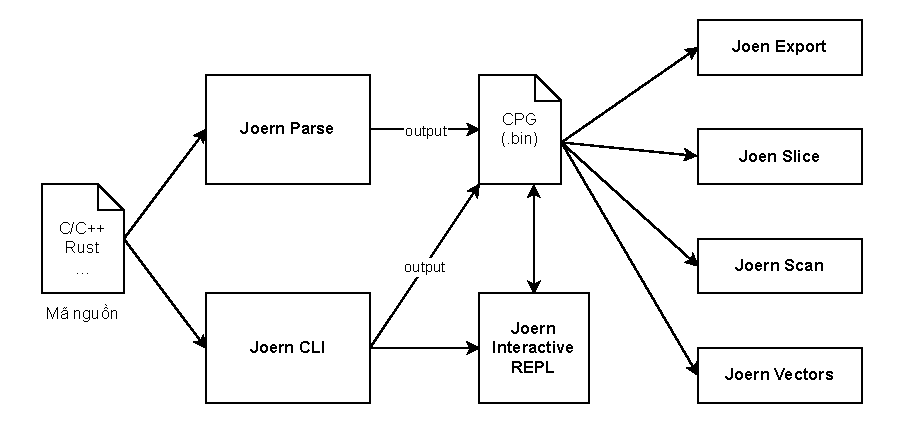
\includegraphics[width=1\columnwidth]{figures/c2/c2_joern_tools.drawio.pdf}
  \centering
  \caption{Các công cụ xung quanh Joern.}
  \label{img:c2_joern_tools}
\end{figure}

Không chỉ cung cấp kiến trúc có tính mở rộng và tái sử dụng cao, Joern còn cung cấp 1 loạt các công cụ để khai thác thông tin từ đồ thị thuộc tính mã nguồn được sinh ra. Các công cụ này bao gồm:

\begin{itemize}
  \item \textbf{JoernExport} chuyển đổi đồ thị thuộc tính mã nguồn từ dạng nhị phân sang dạng dữ liệu tương thích với các cơ sở dữ liệu đồ thị bao gồm neo4jcsv, graphml, graphson, graphviz dot. Từ các định dạng tương thích với cơ sở dữ liệu đồ thị, các ứng dụng về học máy, học tăng cường để phát hiện lỗ hổng trên đồ thị thuộc tính mã nguồn có thể được triển khai \cite{zhou2019devign, alsulami2017source, li2016vulpecker, dauber2018git, machiry2020spider}
  \item \textbf{JoernSlice} cung cấp khả năng chia nhỏ đồ thị CPG của các mã nguồn lớn thành từng phần nhỏ, từ đó dễ dàng khai thác tập trung vào một khía cạnh cụ thể của mã, chẳng hạn như luồng dữ liệu xung quanh một biến cụ thể.
  \item \textbf{JoernScan} thực hiện quét toàn bộ đồ thị thuộc tính để tìm ra lỗ hổng bảo mật. JoernQueryDB \cite{joernJoernQuery} cung cấp cho JoernScan một tập các truy vấn được định nghĩa sẵn để tìm kiếm các mẫu cụ thể trong mã. Các truy vấn trong QueryDB có thể áp dụng riêng cho một ngôn ngữ cụ thể hoặc sử dụng lại chung cho nhiều ngôn ngữ.
  \item \textbf{JoernVectors}: Trích xuất các biểu diễn vectơ từ CPG
\end{itemize}
